%tapered_extension
Moreover, there are other optional designs of tapered waveguide can be involved to improve the Fiber-to-Chip coupling ability. In this section we will only deliver other possibilities of tapered structures for reference and most of them will not be verified in this work.   \\

\textbf{Hybrid tapered waveguides}\\  
In the other simulations of coupling between TLF and tapered waveguide there is another interesting result. If the taper is made from a proper material different from both guide and substrate, a more efficient coupling can be achieved in compare with our previous designs.\\
 
\begin{figure}[!ht]
\centering
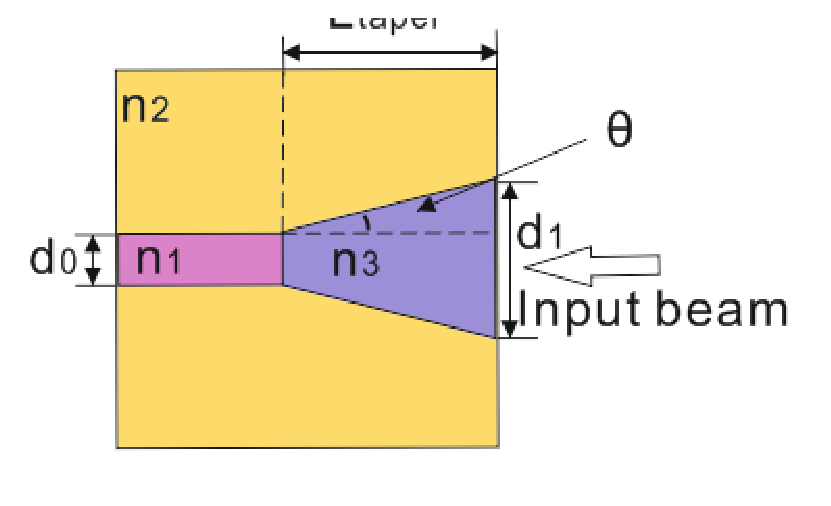
\includegraphics[width=0.7\textwidth]{bilder/tapered_waveguide_others}
\caption{Schema of a tapered waveguide combined with two different materials.}
\label{fig:tapered_waveguide_others}
\end{figure}
For example, for a taper chosen for $n=2.0$, $d_{1}=2\mu$m, $L_{taper}=5.5\mu$m and other configurations maintain as that of the original simulation models. In this case the coupling efficiency reaches $|S_{21}|=63\%$ according the simulation result Fig. \ref{fig:tapered_waveguide_others_coupling}.  Because this design is not easy for fabrication, no more attention will be paid on it in this section.\\
   
\begin{figure}[!ht]
\centering
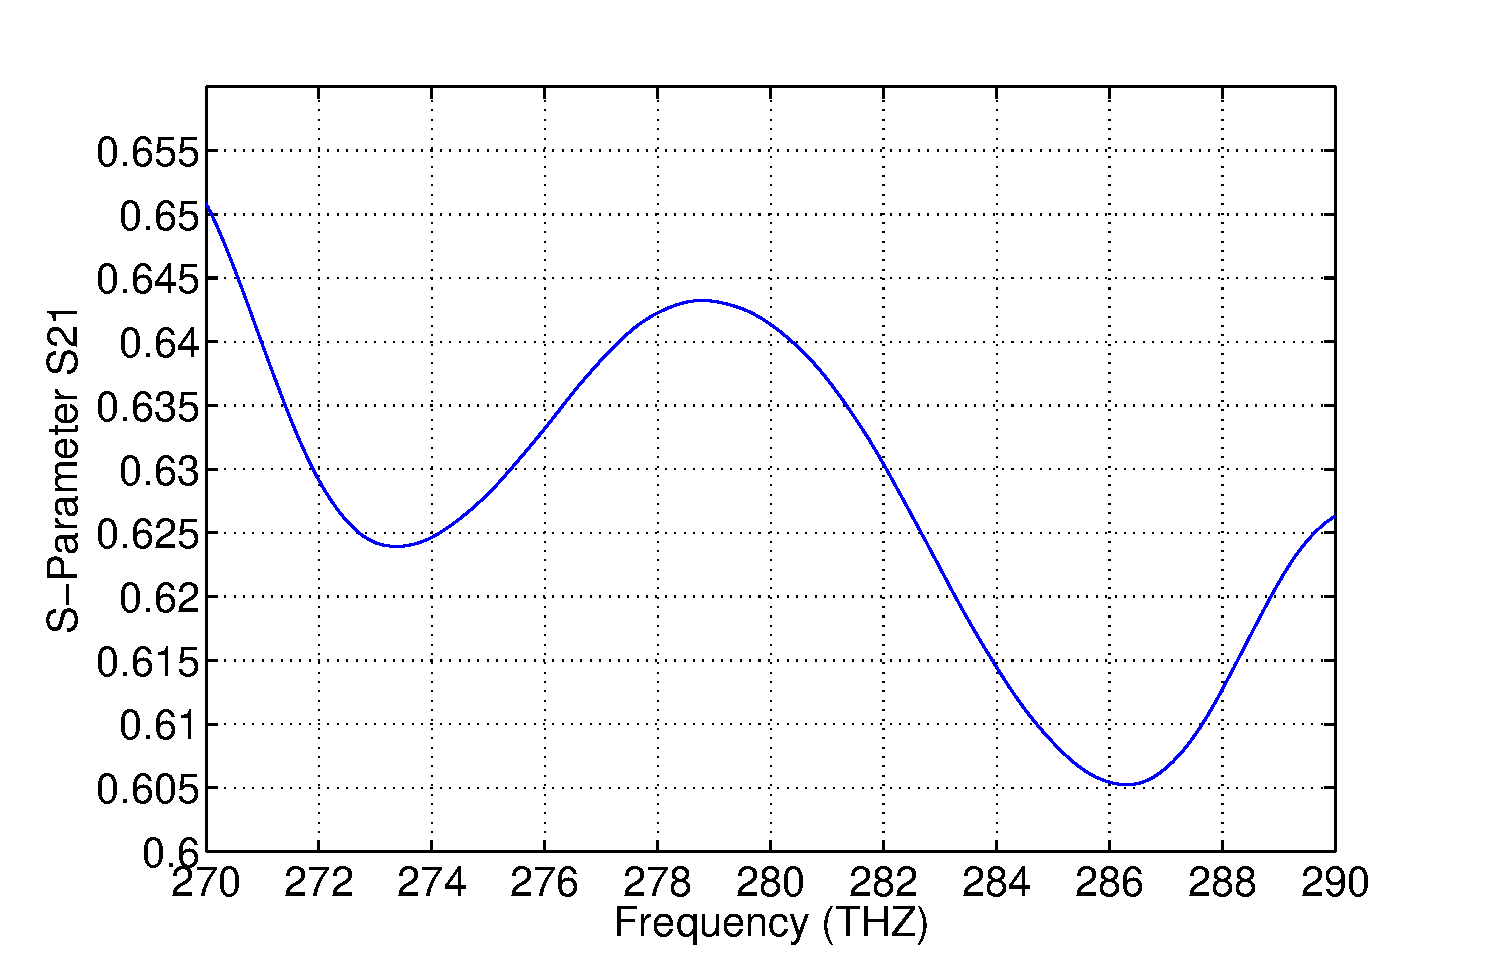
\includegraphics[width=0.7\textwidth]{bilder/s21_tapered_waveguide_others}
\caption{Coupling efficiency between TLF and the tapered waveguide combined with two different materials.}
\label{fig:tapered_waveguide_others_coupling}
\end{figure}
\textbf{Tapered plasmonic waveguides}\\
Verhagen mentions in \cite{tapered_plasmonic_waveguides} a tapered plasmonic waveguide, which is composed of a thin tapered metal film, on the surface of which lies many small holes like Fig. \ref{fig:tapered_waveguide_plasmonic}. For transmission input beams excite the surface plasmon polariton (SPP) wave, which is explained by quantum emission, provided by the metal/dielectric interfaces of the plasmonic waveguides. By means of this arrangement the coupling efficiency can even achieve a value greater than $100\%$. \\

\begin{figure}[!ht]
\centering
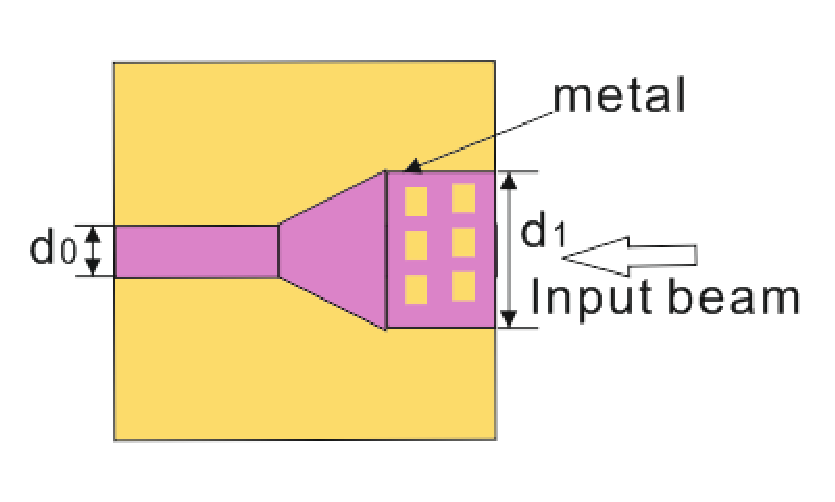
\includegraphics[width=0.7\textwidth]{bilder/tapered_waveguide_plasmonic}
\caption{Schema of a taperd plasmonic waveguide.}
\label{fig:tapered_waveguide_plasmonic}
\end{figure}
\textbf{Grating tapered waveguides}\\
Alonso-Ramos has provided in \cite{fiber_to_chip_grating_waveguides} an inversely tapered waveguide with gratings like Fig. \ref{fig:tapered_waveguide_grating}. The gratings of this waveguide are delicately designed to match the work mode: bloch mode. In \cite{fiber_to_chip_grating_waveguides} the author presented his achievement of $65.6\%$ coupling efficiency. \\
 
\begin{figure}[!ht]
\centering
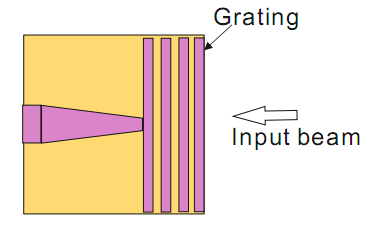
\includegraphics[width=0.7\textwidth]{bilder/tapered_waveguide_grating}
\caption{Schema of a taperd waveguide with grating.}
\label{fig:tapered_waveguide_grating}
\end{figure}
